\documentclass[12pt]{beamer}
\usepackage[utf8]{inputenc}
\usepackage[T1]{fontenc}
\usepackage{lmodern}
\usetheme{Malmoe}
%\usetheme{Warsaw}

\newcommand{\tc}[1]{
	\textcolor{blue}{#1}
}

\usepackage{graphicx}

\begin{document}
	\author{Lukáš Růžicka}
	\title{Modularita ve Fedoře 29}
	\subtitle{}
	\titlegraphic{
\includegraphics[width=3cm]{logo.png}}
	\logo{
\includegraphics[width=1cm]{logo.png}}
	\institute{Fedora 29 Release}
	\date{listopad 2018}
	\subject{Fedora 29}
	%\setbeamercovered{transparent}
	%\setbeamertemplate{navigation symbols}{}
	\begin{frame}[plain]
	\maketitle
\end{frame}

\begin{frame}
\frametitle{Modularita pro všechny}
Do \textbf{Fedory 29} přichází globální podpora pro modularitu, kterou jsme zatím mohli potkat pouze ve \textbf{Fedora Server 28}. 

Nyní ve verzi 29, modularita:

\vspace{5pt}

\begin{enumerate}
	\item je zapnutá napříč spiny
	\item je zatím dobrovolná
	\item pokrývá pouze malé spektrum aplikací (cca 30)
	\item je rámcově funkční
\end{enumerate}	
\end{frame}


\section{Co je modularita?}

\begin{frame}
\frametitle{Co je vlastně modularita?}


\begin{itemize}
	\item nový plán na poskytování aplikací
	\item řeší problémy tradiční distribuce software
	\item větší přizpůsobení se uživatelským potřebám
\end{itemize}

\end{frame}

\begin{frame}
\frametitle{Přehled modulárního OS}

\begin{center}
	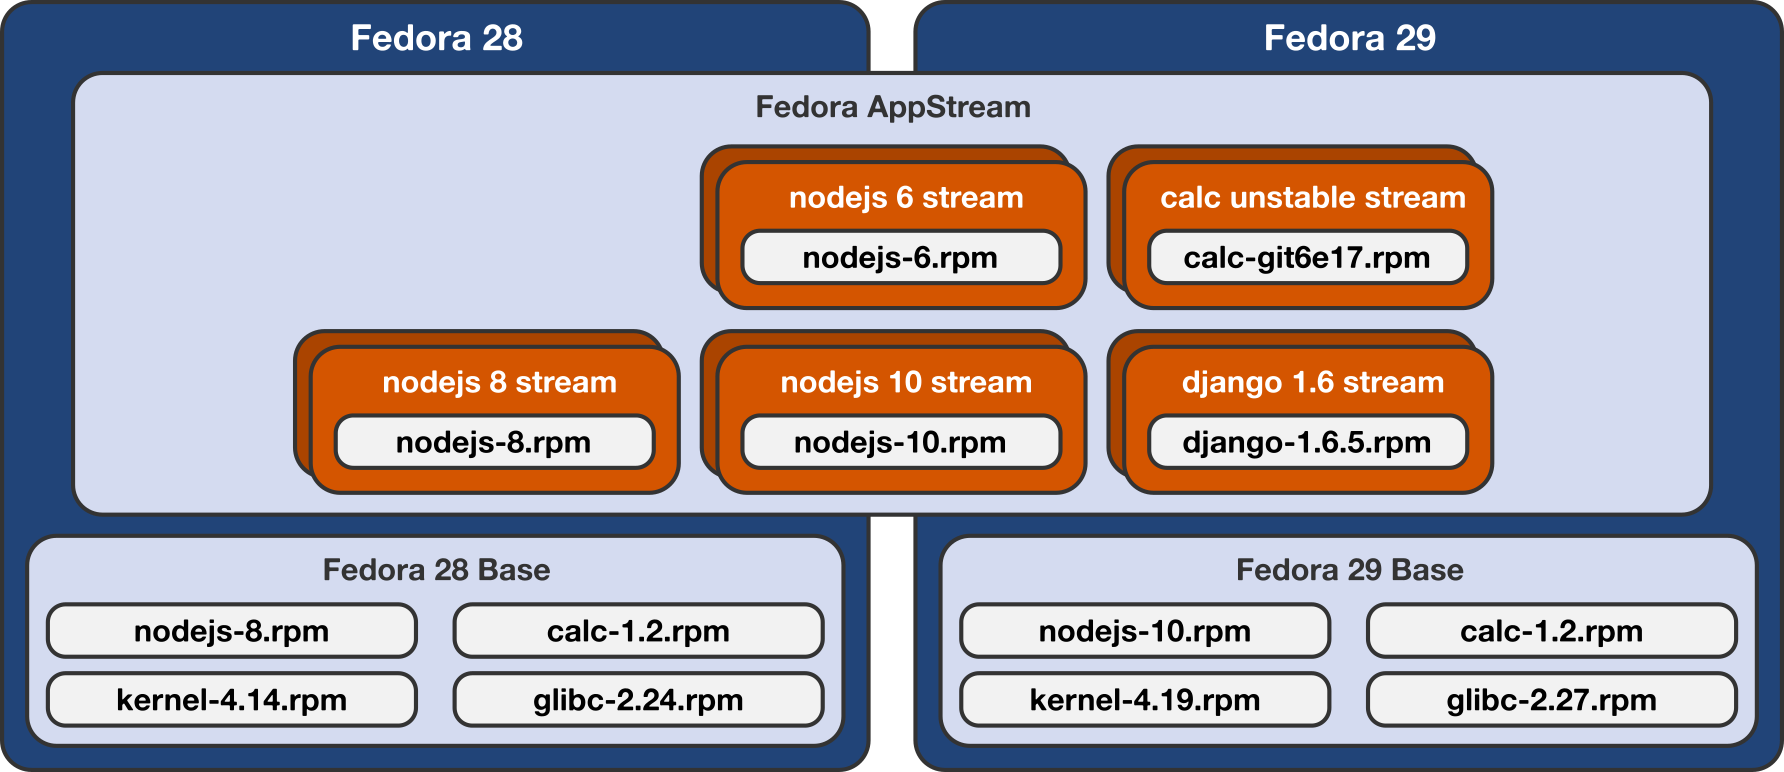
\includegraphics[width=10cm]{overview}
\end{center}
\end{frame}

\begin{frame}
\frametitle{Co pro vás může modularita udělat?}
Nejdiskutovanější případy použití, které modularita pro uživatele řeší, jsou:

\vspace{5pt}

\begin{itemize}
	\item standardní vývoj Fedory je příliš \textit{pomalý} nebo \textit{rychlý}
	\item lepší použití v kontejnerovém prostředí
	\item snadnější správa balíčků
\end{itemize}
\end{frame}

\section{Správa software a modularita}

\begin{frame}
\frametitle{Tradiční pojetí balíčků}
V tradičním pojetí se balíčky vytvářejí z jedné verze zdrojových kódů pro určitou verzi Fedory. V pozdějších verzích Fedory se objevují novější balíčky.
\begin{center}
	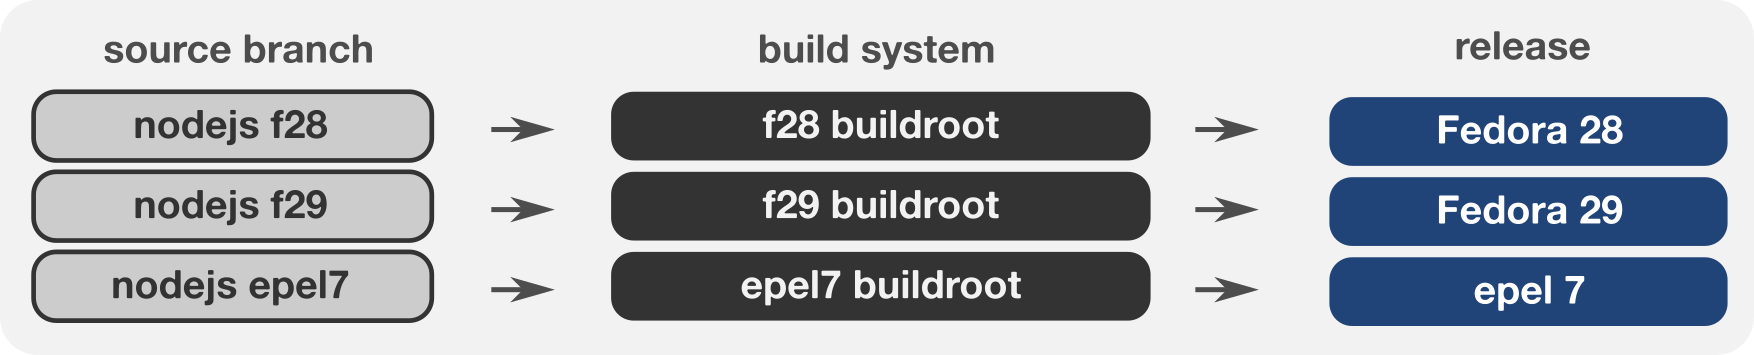
\includegraphics[width=10cm]{traditional}
\end{center}
\end{frame}

\begin{frame}
\frametitle{Modulární pojetí balíčků}
V \textit{modulárním} pojetí se balíčky vytvářejí z jedné verze zdrojových kódů pro různé verze Fedory. Jednotlivé verze balíčků mohou být dostupné v několika verzích Fedory.
\begin{center}
	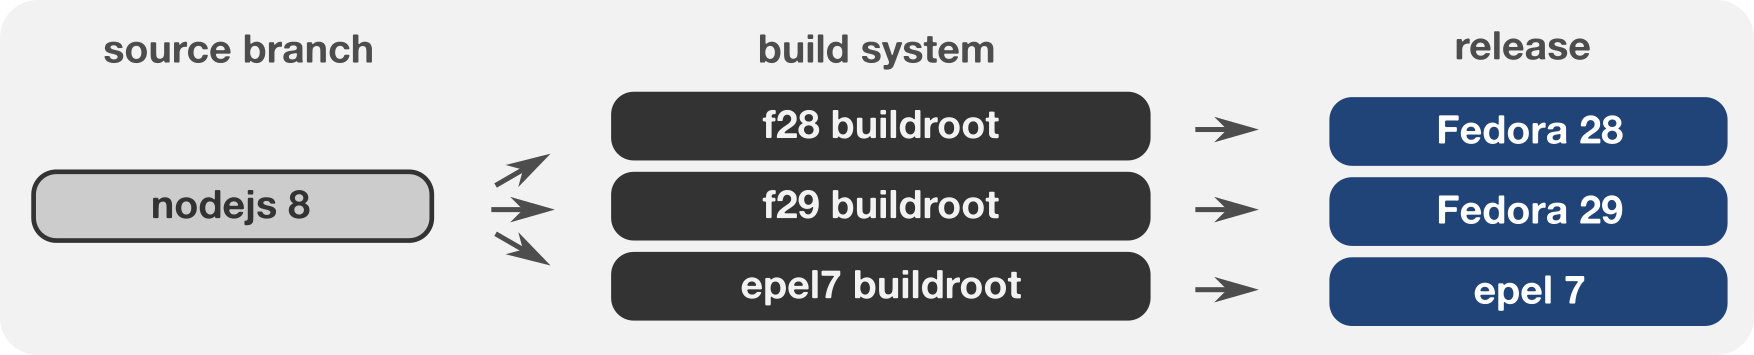
\includegraphics[width=10cm]{modular}
\end{center}
\end{frame}

\begin{frame}
\frametitle{Jedna verze balíčků, více verzí Fedory}
Modul může být nastaven tak, aby se balíček přeložil pro několik verzí Fedory najednou. 

\begin{center}
	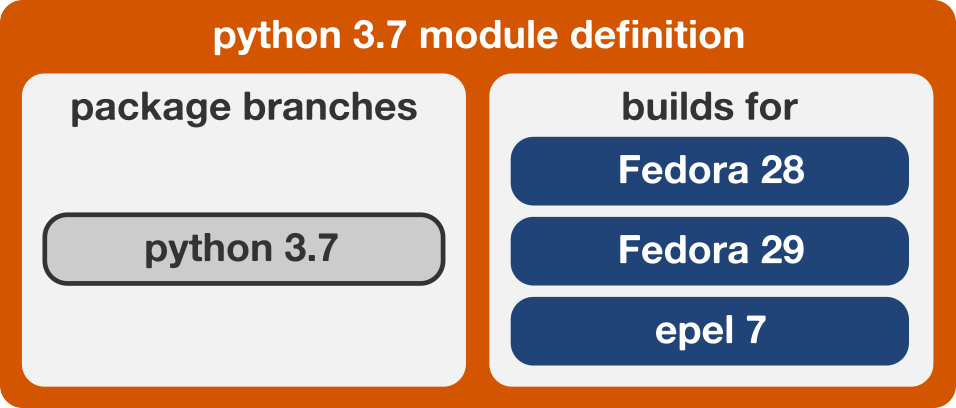
\includegraphics[width=7cm]{forversion}
\end{center}
\end{frame}

\begin{frame}
\frametitle{Více verzí balíčků, jedna verze Fedory}
Moduly lze využít i tak, že pro jednu verzi Fedory se přeloží několik různých verzí příslušného software.

\begin{center}
	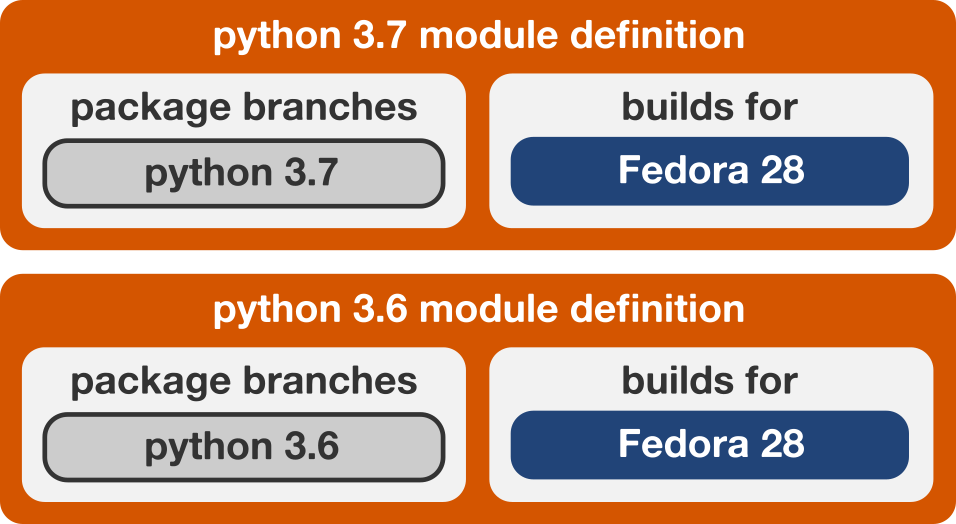
\includegraphics[width=7cm, height=3.5cm]{multiversion}
\end{center}

Modulární přístup však nedovoluje mít v systému více verzí jedné aplikace, bez použití dalších technologií (kontejner).

\end{frame}

\begin{frame}
\frametitle{Složitější strategie}
Moduly lze také přeložit oproti dalším modulům a tak je možné vyřešit i daleko komplexnější požadavky uživatelů.

\begin{center}
	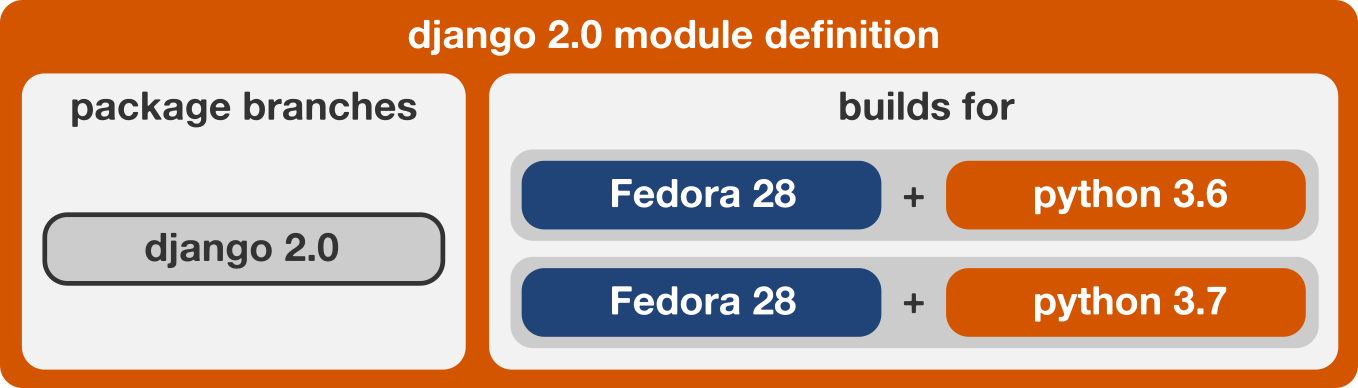
\includegraphics[width=8cm]{combined}
\end{center}
\end{frame}

\begin{frame}
\frametitle{Organizace repozitářů}

\begin{enumerate}
	\item tradiční repozitář
	\item modulární repozitář (AppStream)
\end{enumerate}

\begin{center}
	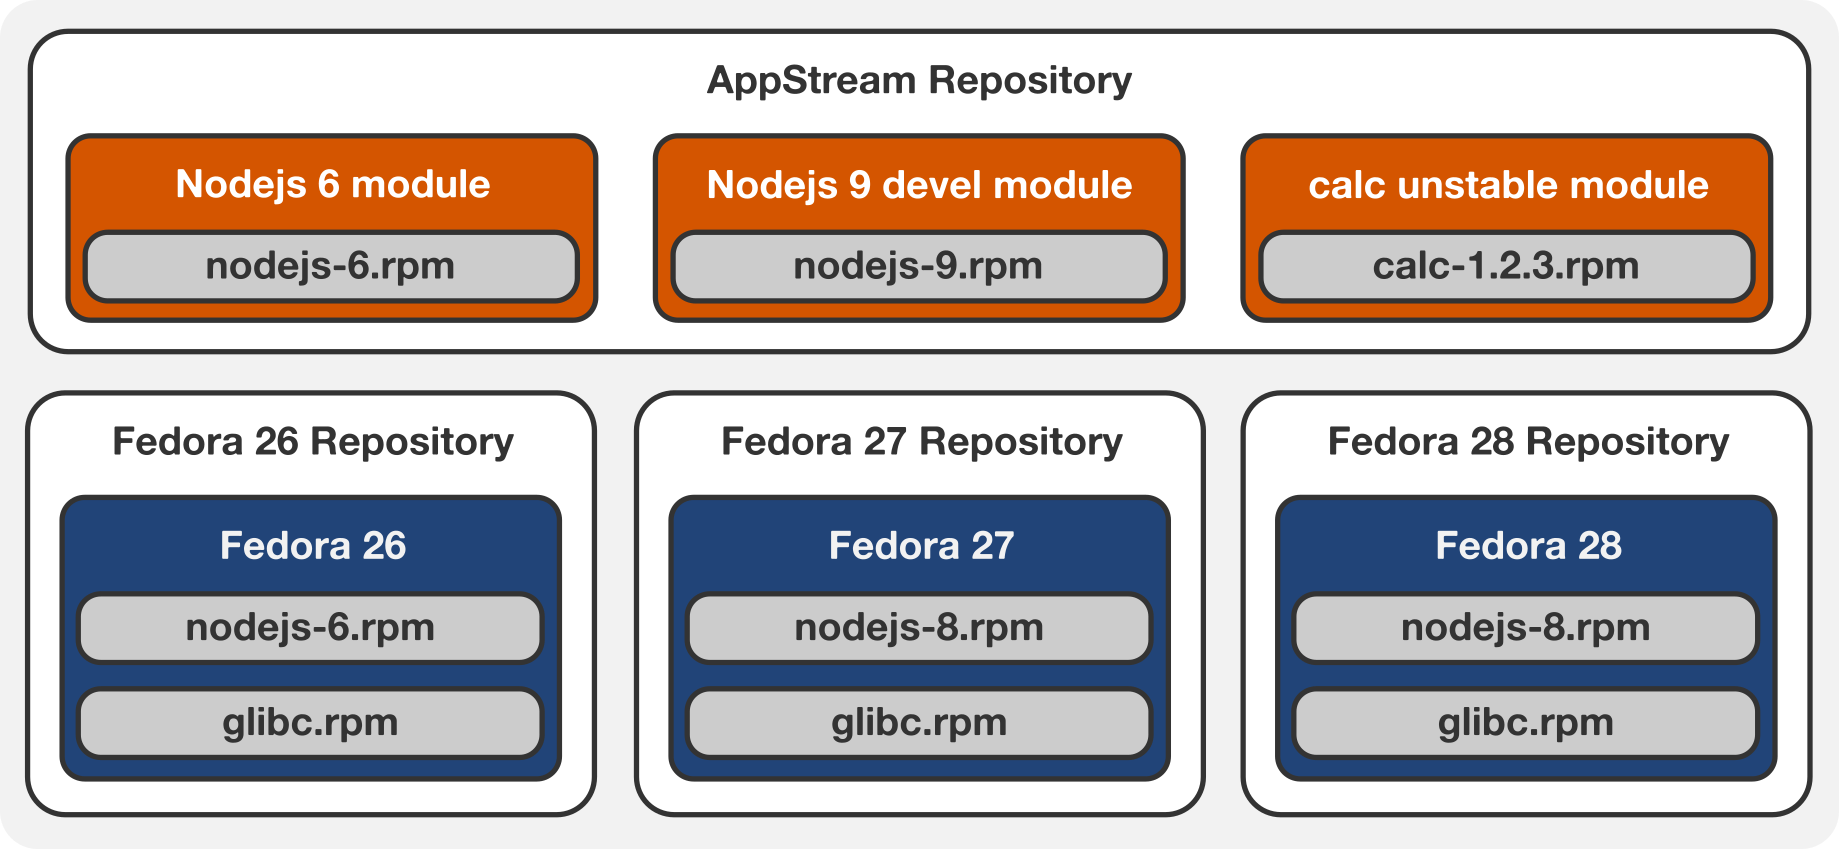
\includegraphics[width=10cm]{repos}
\end{center}
\end{frame}

\begin{frame}
\frametitle{Modulární repozitáře ve Fedoře 29}

\begin{enumerate}
	\item fedora-modular.repo
	\item fedora-updates-modular.repo
	\item fedora-updates-testing-modular.repo
\end{enumerate}

\begin{center}
	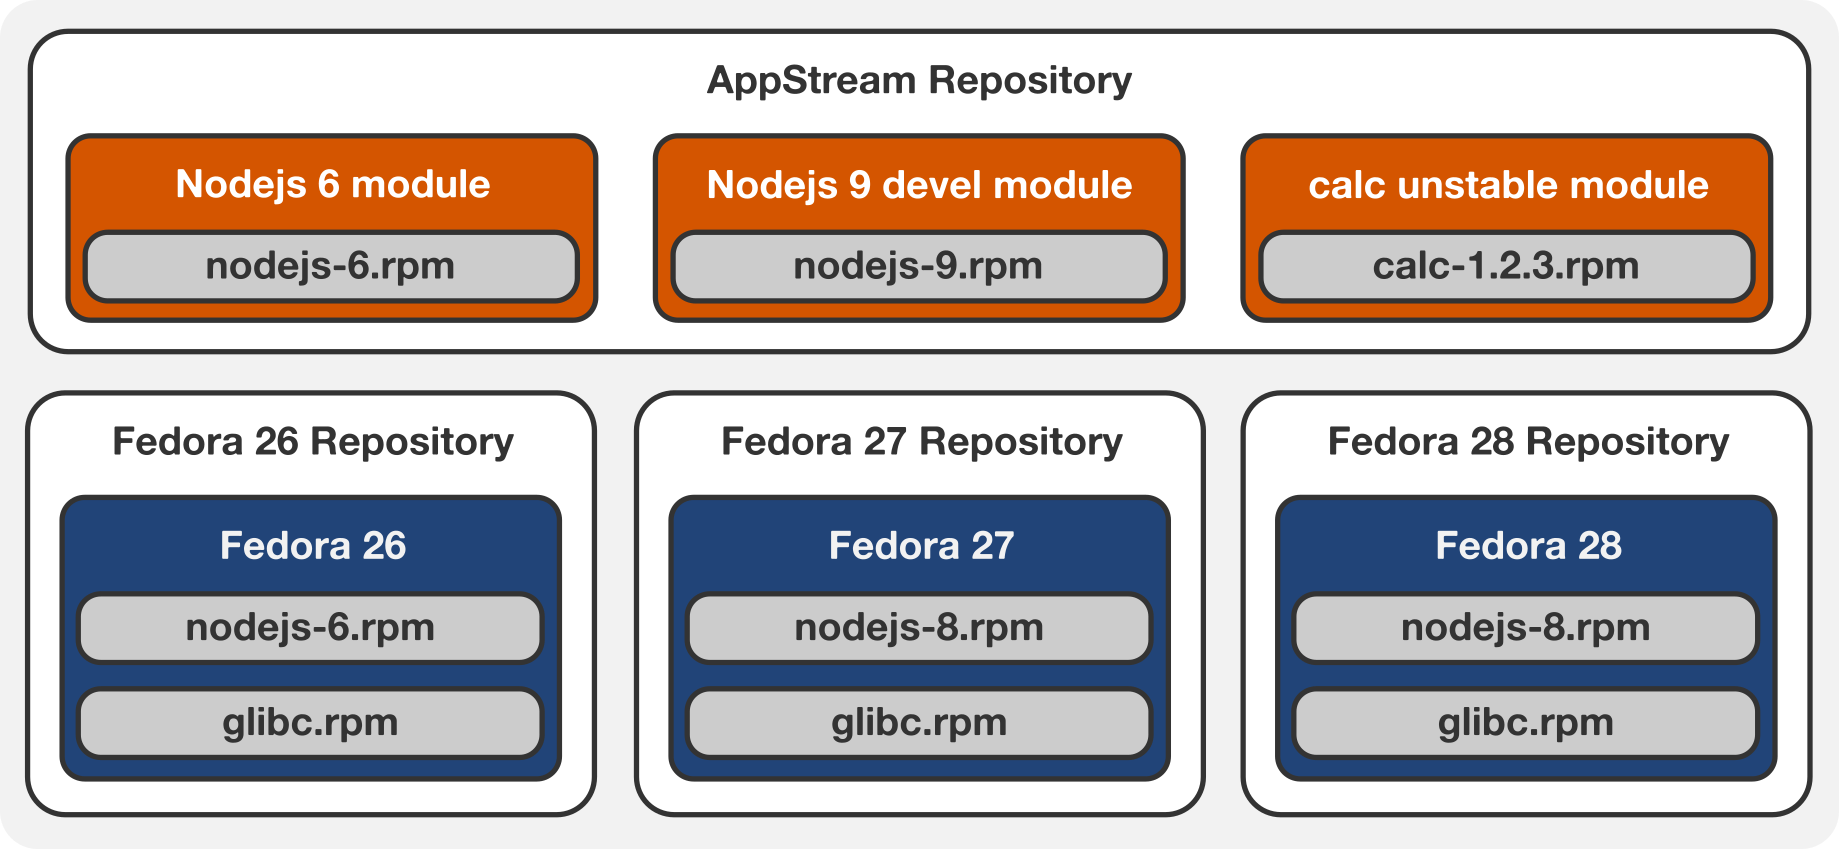
\includegraphics[width=9cm]{repos}
\end{center}
\end{frame}

\begin{frame}
\frametitle{Modulární repozitáře ve Fedoře 29}

\begin{enumerate}
	\item umístění v \textcolor{blue}{\texttt{/etc/yum.repos.d/}}
	\item standartně povolené
\end{enumerate}
\end{frame}

\section{Používání modulárního obsahu}

\begin{frame}
\frametitle{Práce s modulem}

K používání modulárního obsahu existuje několik operací:

\begin{enumerate}
	\item zobrazit seznam modulů
	\item povolit modul
	\item nainstalovat modul
	\begin{itemize}
		\item stream
		\item profile
	\end{itemize}
	\item změnit \textit{stream} modulu
	\item odinstalovat modul
	\item zakázat modul
\end{enumerate}
\end{frame}

\begin{frame}
\frametitle{Zobrazení seznamu dostupných modulů}

Zobrazení seznamu všech dostupných modulů:

\begin{center}
	\tc{\texttt{dnf module list}}
\end{center}

Informace o konkrétním modulu:

\begin{center}
	\tc{\texttt{dnf module list <modulename>}}
\end{center}
\end{frame}

\begin{frame}
\frametitle{Další možnosti zobrazení}

Zobrazení seznamu všech dostupných modulů:

\begin{center}
	\tc{\texttt{dnf module list -\,-enabled}}
	
	\tc{\texttt{dnf module list -\,-disabled}}
	
	\tc{\texttt{dnf module list -\,-installed}}	
\end{center}
\end{frame}

\end{document}